\documentclass{article}

  % packages
    % basic stuff for rendering math
    \usepackage[letterpaper, top=1in, bottom=1in, left=1in, right=1in]{geometry}
    \usepackage[english]{babel}
    \usepackage{amsmath, amssymb} 
    \usepackage{bbm}              % for mathbbm

    % extra math symbols and utilities
    \usepackage{mathtools}        % for extra stuff like \coloneqq
    \usepackage{mathrsfs}         % for extra stuff like \mathsrc{}
    \usepackage{centernot}        % for the centernot arrow 
    \usepackage{bm}               % for better boldsymbol/mathbf 
    \usepackage{enumitem}         % better control over enumerate, itemize
    \usepackage{xr-hyper}	  % for external links
    \usepackage{hyperref}         % for hypertext linking
    \usepackage{fancyvrb}         % for better verbatim environments
    \usepackage{newverbs}         % for texttt{}
    \usepackage{xcolor}           % for colored text 
    \usepackage{listings}         % to include code
    \usepackage{lstautogobble}    % helper package for code
    \usepackage{parcolumns}       % for side by side columns for two column code
    \usepackage{algorithm} 	  % for algorithm pseudocode
    \usepackage{algpseudocode}	  % for algorithm pseudocode
    

    % page layout
    \usepackage{fancyhdr}         % for headers and footers 
    \usepackage{lastpage}         % to include last page number in footer 
    \usepackage{parskip}          % for no indentation and space between paragraphs    
    \usepackage[T1]{fontenc}      % to include \textbackslash
    \usepackage{footnote}
    \usepackage{etoolbox}

    % for custom environments
    \usepackage{tcolorbox}        % for better colored boxes in custom environments
    \tcbuselibrary{breakable}     % to allow tcolorboxes to break across pages

    % figures and tables 
    \usepackage{pgfplots}
    \pgfplotsset{compat=1.18}
    \usepackage{float}            % for [H] figure placement
    \usepackage{tikz, tikz-cd}
    \usetikzlibrary{arrows, positioning, calc}
    \usepackage{graphicx}
    \usepackage{caption, subcaption} 
    \usepackage{dcolumn}

    \usepackage[nottoc]{tocbibind}
    \hfuzz=5.002pt                % ignore overfull hbox badness warnings below this limit

  % New and replaced operators
    \DeclareMathOperator{\std}{std}
    \DeclareMathOperator*{\argmin}{\arg\!\min}
    \DeclareMathOperator*{\argmax}{\arg\!\max}
    \newcommand{\ket}[1]{\ensuremath{\left|#1\right\rangle}}
    \newcommand{\bra}[1]{\ensuremath{\left\langle#1\right|}}
    \newcommand{\braket}[2]{\langle #1 | #2 \rangle}
    \newcommand{\qed}{$\blacksquare \quad$}     % I like QED squares to be black

  % Custom Environments
    \tcbset{
      colframe = black,
      colback  = white,
      coltitle = black,
      colbacktitle = black!10,
      breakable, 
      arc=0mm,
      boxrule=1pt,
      left=8pt,
      right=8pt,
      top=6pt,
      bottom=6pt,
      before skip=12pt,
      after skip=12pt,
      bottomrule at break=-1pt,
      toprule at break=-1pt,
      fonttitle=\bfseries,
    }
    \newcounter{question}
    \renewcommand{\thequestion}{\arabic{question}}
    \NewDocumentEnvironment{question}{O{} o}{%
      \refstepcounter{question}%
      \ifstrempty{#1}{%
        \begin{tcolorbox}[title=\textbf{Question \thequestion}]%
      }{%
        \IfValueTF{#2}{%
          \begin{tcolorbox}[title=\textbf{Question \thequestion~(#1)}, label={#2}]%
        }{%
          \begin{tcolorbox}[title=\textbf{Question \thequestion~(#1)}]%
        }%
      }%
    }{%
      \end{tcolorbox}%
    }

    \newcounter{exercise}
    \renewcommand{\theexercise}{\arabic{exercise}}
    \NewDocumentEnvironment{exercise}{O{} o}{%
      \refstepcounter{exercise}%
      \ifstrempty{#1}{%
        \begin{tcolorbox}[title=\textbf{Exercise \theexercise}]%
      }{%
        \IfValueTF{#2}{%
          \begin{tcolorbox}[title=\textbf{Exercise \theexercise~(#1)}, label={#2}]%
        }{%
          \begin{tcolorbox}[title=\textbf{Exercise \theexercise~(#1)}]%
        }%
      }%
    }{%
      \end{tcolorbox}%
    }

    \newtcolorbox[auto counter, number within=section]{solution}[1][]
    {
      before skip = -7pt,
      before upper = \textit{Solution. },
    }

    \newcounter{theorem}[section]
    \renewcommand{\thetheorem}{\thesection.\arabic{theorem}}

    \NewDocumentEnvironment{lemma}{O{} o}{%
      \refstepcounter{theorem}%
      \ifstrempty{#1}{%
        \begin{tcolorbox}[title=\textbf{Lemma \thetheorem}]%
      }{%
        \IfValueTF{#2}{%
          \begin{tcolorbox}[title=\textbf{Lemma \thetheorem~(#1)}, label={#2}]%
        }{%
          \begin{tcolorbox}[title=\textbf{Lemma \thetheorem~(#1)}]%
        }%
      }%
    }{%
      \end{tcolorbox}%
    }

    \NewDocumentEnvironment{theorem}{O{} o}{%
      \refstepcounter{theorem}%
      \ifstrempty{#1}{%
        \begin{tcolorbox}[title=\textbf{Theorem \thetheorem}]%
      }{%
        \IfValueTF{#2}{%
          \begin{tcolorbox}[title=\textbf{Theorem \thetheorem~(#1)}, label={#2}]%
        }{%
          \begin{tcolorbox}[title=\textbf{Theorem \thetheorem~(#1)}]%
        }%
      }%
    }{%
      \end{tcolorbox}%
    }

    \NewDocumentEnvironment{corollary}{O{} o}{%
      \refstepcounter{theorem}%
      \ifstrempty{#1}{%
        \begin{tcolorbox}[title=\textbf{Corollary \thetheorem}]%
      }{%
        \IfValueTF{#2}{%
          \begin{tcolorbox}[title=\textbf{Corollary \thetheorem~(#1)}, label={#2}]%
        }{%
          \begin{tcolorbox}[title=\textbf{Corollary \thetheorem~(#1)}]%
        }%
      }%
    }{%
      \end{tcolorbox}%
    }

    \newtcolorbox[auto counter, number within=section]{proof}[1][]
    {
      before skip = -7pt,
      before upper = \textit{Proof. },
    }

    \newcounter{definition}[section]
    \renewcommand{\thedefinition}{\thesection.\arabic{definition}}
    \NewDocumentEnvironment{definition}{O{} o}{%
      \refstepcounter{definition}%
      \ifstrempty{#1}{%
        \begin{tcolorbox}[title=\textbf{Definition \thedefinition}]%
      }{%
        \IfValueTF{#2}{%
          \begin{tcolorbox}[title=\textbf{Definition \thedefinition~(#1)}, label={#2}]%
        }{%
          \begin{tcolorbox}[title=\textbf{Definition \thedefinition~(#1)}]%
        }%
      }%
    }{%
      \end{tcolorbox}%
    }

    \newcounter{example}[section]
    \renewcommand{\theexample}{\thesection.\arabic{example}}
    \NewDocumentEnvironment{example}{O{} o}{%
      \refstepcounter{example}%
      \ifstrempty{#1}{%
        \begin{tcolorbox}[title=\textbf{Example \theexample}]%
      }{%
        \IfValueTF{#2}{%
          \begin{tcolorbox}[title=\textbf{Example \theexample~(#1)}, label={#2}]%
        }{%
          \begin{tcolorbox}[title=\textbf{Example \theexample~(#1)}]%
        }%
      }%
    }{%
      \end{tcolorbox}%
    }

    \newcounter{code}[section]
    \renewcommand{\thecode}{\thesection.\arabic{code}}
    \NewDocumentEnvironment{code}{O{} o}{%
      \refstepcounter{code}%
      \ifstrempty{#1}{%
        \begin{tcolorbox}[title=\textbf{Code \thecode}]%
      }{%
        \IfValueTF{#2}{%
          \begin{tcolorbox}[title=\textbf{Code \thecode~(#1)}, label={#2}]%
        }{%
          \begin{tcolorbox}[title=\textbf{Code \thecode~(#1)}]%
        }%
      }%
    }{%
      \end{tcolorbox}%
    } 

    \definecolor{dkgreen}{rgb}{0,0.6,0}
    \definecolor{gray}{rgb}{0.5,0.5,0.5}
    \definecolor{mauve}{rgb}{0.58,0,0.82}
    \definecolor{lightgray}{gray}{0.93}

    % default options for listings (for code)
    \lstset{
      autogobble,
      frame=ltbr,
      language=C,                           % the language of the code
      aboveskip=3mm,
      belowskip=3mm,
      showstringspaces=false,
      columns=fullflexible,
      keepspaces=true,
      basicstyle={\small\ttfamily},
      numbers=left,
      firstnumber=1,                        % start line number at 1
      numberstyle=\tiny\color{gray},
      keywordstyle=\color{blue},
      commentstyle=\color{dkgreen},
      stringstyle=\color{mauve},
      backgroundcolor=\color{lightgray}, 
      breaklines=true,                      % break lines
      breakatwhitespace=true,
      tabsize=3, 
      xleftmargin=2em, 
      framexleftmargin=1.5em, 
      stepnumber=1
    }

  % Page style
    \pagestyle{fancy}
    \fancyhead[L]{}
    \fancyhead[C]{Muchang Bahng}
    \fancyhead[R]{Fall 2026} 
    \fancyfoot[C]{\thepage / \pageref{LastPage}}
    \renewcommand{\footrulewidth}{0.4pt}          % the footer line should be 0.4pt wide
    \renewcommand{\thispagestyle}[1]{}  % needed to include headers in title page

  % external documents 
  % \externaldocument[st-]{../../Math/Set\_Theory/paper}[https://mbahng.com/Math/Set\_Theory/paper.pdf] 

\begin{document}

\title{PS 1}
\author{Muchang Bahng}
\date{Fall 2026}

\maketitle

\begin{exercise}
  In the 2020 US Presidential election, there was a significant gap between the probability of a Biden victory assigned by poll aggregators (e.g., fivethirtyeight.com) and betting markets. According to Bayesian decision theory, a rational agent should choose actions (in this case, bet size) by writing down:
  \begin{itemize}
    \item a probability distribution $P(X)$ over the state $X$ of the world describing what they think will happen,
    \item a utility function $U$ describing the value of each action under a certain state of the world,
  \end{itemize}
  and then choose the action that maximizes their expected utility (equivalently, minimizes expected risk). That is, a rational agent will choose
  \[
    a^* = \argmax_a \mathbb{E}_{X \sim P}\left[U(a, X)\right].
  \]
  Suppose that Victor is a rational agent with $d$ dollars of total wealth, and that he thinks $P(\text{Biden wins}) = 0.85$ (the fivethirtyeight prediction), and that betting markets give even money bets at $P(\text{Biden wins}) = 0.6$.
  \begin{enumerate}[label=(\alph*)]
    \item Prove that if Victor's utility function is just the amount of money he has then he'll bet $d$ (his entire bankroll) on Biden winning. Does this kind of linear utility of money make sense?
    \item Now, suppose that Victor's utility from $y$ dollars is simply $U(y) = \log(y)$. How much (of his $d$ dollars) should he bet on Biden winning?
    \item Suppose you had a net worth of \$500,000. Would you personally make the bet from part (b)?
  \end{enumerate}
\end{exercise}
\begin{solution}
  Throughout, a bet of size $x \in [0,d]$ on Biden at market probability $q = 0.6$ pays a profit of $b x$ with $b = \frac{1-q}{q} = \frac{2}{3}$ if Biden wins, and loses $x$ otherwise. Let $p = 0.85$ be Victor's belief.

  \begin{enumerate}[label=(\alph*)]
    \item With $U(y) = y$, the final wealth is $d + bx$ with probability $p$ and $d - x$ with probability $1-p$, so
      \[
        \mathbb{E}[U(x, X)] = p(d + bx) + (1-p)(d - x) = d + x\big(pb - (1-p)\big) = d + x\left(0.85 \cdot \tfrac{2}{3} - 0.15\right) = d + \tfrac{5}{12}x .
      \]
      This is strictly increasing in $x$, so the maximizer over $x \in [0,d]$ is $x^* = d$: he bets his entire bankroll. In general, $x^* = d$ whenever $pb > 1-p$, i.e.\ $p > q$.

      Linear utility of money does not make sense: it says that Victor is indifferent between $\$1$ for sure and a $50\%$ chance of $\$2$, and would risk ruin (a $15\%$ chance of losing everything) for an expected gain of $\frac{5}{12}d$. It ignores the diminishing marginal value of money and the fact that losing all wealth is catastrophic.

    \item Now maximize
      \[
        g(x) = p \log(d + bx) + (1-p)\log(d - x), \qquad x \in [0, d).
      \]
      $g$ is strictly concave, and $g(x) \to -\infty$ as $x \to d$, so the maximizer is interior and is given by $g'(x) = 0$:
      \[
        \frac{pb}{d + bx} = \frac{1-p}{d-x}
        \Longrightarrow pb(d-x) = (1-p)(d+bx)
        \Longrightarrow x b = d\big(pb - (1-p)\big)
        \Longrightarrow x^* = d\left(p - \frac{1-p}{b}\right).
      \]
      (This is the Kelly criterion.) Plugging in, $x^* = d\left(0.85 - \frac{0.15}{2/3}\right) = d(0.85 - 0.225) = 0.625\,d$. So Victor should bet $62.5\%$ of his wealth.

    \item With $d = \$500{,}000$, the Kelly bet is $\$312{,}500$. Personally I would not make this bet. The calculation takes the $0.85$ forecast as exactly correct, but if the forecast is overconfident (the market is saying $0.6$, and the market has money on the line), the optimal bet shrinks quickly; e.g.\ with $p = 0.6$ the optimal bet is $0$. Kelly is also known to be aggressive: it is very sensitive to errors in $p$ and to model misspecification. Furthermore, a $15\%$ chance of losing $\$312{,}500$ (over half of my net worth) is a risk I would not take in a single event, and my true utility over this range is more risk averse than $\log$. A fractional Kelly bet would be more reasonable.
  \end{enumerate}
\end{solution}

\begin{exercise}
  Suppose that $Y$ is a categorical random variable, and $X$ are covariates that we wish to use to predict $Y$. A loss function $L$ on categorical data is called a \textit{proper scoring rule} if the predictive function $f^*$ that minimizes the implied risk is the conditional probability of $Y$ given $X$. That is, if
  \[
    f^* \coloneqq \argmin_f \mathbb{E}_{X,Y}\left[L\left(Y, f(X)\right)\right] \text{ is given by } f^*(x) = P(Y \mid X = x).
  \]
  Prove that the Cross Entropy loss is a proper scoring rule in the case where $Y$ is binary.
\end{exercise}
\begin{solution}
  Let $Y \in \{0,1\}$ and let $f(x) \in (0,1)$ denote the predicted probability that $Y = 1$. The cross entropy loss is $L(y, f(x)) = -\big[y \log f(x) + (1-y)\log(1 - f(x))\big]$. By the tower property,
  \[
    \mathbb{E}_{X,Y}[L(Y, f(X))] = \mathbb{E}_X\Big[\mathbb{E}_{Y \mid X}\big[L(Y, f(X))\big]\Big],
  \]
  so the risk is minimized by minimizing the inner conditional expectation separately at each $x$ (we can choose the value $f(x)$ freely for each $x$). Fix $x$ and let $p = P(Y = 1 \mid X = x)$ and $q = f(x)$. Then
  \[
    \phi(q) \coloneqq \mathbb{E}[L(Y,q) \mid X = x] = -p\log q - (1-p)\log(1-q).
  \]
  Differentiating,
  \[
    \phi'(q) = -\frac{p}{q} + \frac{1-p}{1-q} = \frac{q - p}{q(1-q)},
  \]
  which is negative for $q < p$ and positive for $q > p$ (when $p \in (0,1)$). Hence $\phi$ is strictly decreasing and then strictly increasing, with unique minimizer $q = p$. (Equivalently, $\phi(q) = H(p) + \mathrm{KL}(\mathrm{Ber}(p)\,\|\,\mathrm{Ber}(q)) \ge H(p)$, with equality iff $q = p$.) If $p = 0$ or $1$, $\phi(q) = -\log(1-q)$ or $-\log q$, which is minimized (as an infimum) at $q = p$ as well.

  Therefore the pointwise minimizer is $f^*(x) = P(Y = 1 \mid X = x)$ for every $x$, so $f^* = \argmin_f \mathbb{E}[L(Y, f(X))]$ is the conditional probability, and cross entropy is a proper scoring rule. \qed
\end{solution}

\begin{exercise}
  As we saw in class, a requirement for stochastic gradient descent to converge to the minimum of an objective function is that the step size $\rho_t$ decays fast enough that $\sum_t \rho_t^2 < \infty$. In actual machine learning practice, it's a common practice to just use a constant step size, violating the convergence requirement. Why might this be reasonable in a finite sample setting?
\end{exercise}
\begin{solution}
  The condition $\sum_t \rho_t^2 < \infty$ (together with $\sum_t \rho_t = \infty$) is what kills the gradient noise so that SGD converges exactly to the minimizer of the objective. In practice this is not what we want, for several reasons.
  \begin{enumerate}
    \item \textbf{Finite compute.} We only run a finite number $T$ of steps, so $\sum_{t \le T} \rho^2 = T\rho^2 < \infty$ trivially; the asymptotic condition is never actually tested. Meanwhile, a decaying schedule like $\rho_t \sim 1/t$ shrinks so quickly that progress is very slow in the time budget we actually have, whereas a constant step size makes (for strongly convex smooth objectives) geometric progress toward the minimizer until it reaches a noise floor.
    \item \textbf{The noise floor is of the same order as the statistical error.} With constant step size $\rho$, SGD converges linearly to a neighborhood of the minimizer whose radius is $O(\rho\sigma^2)$ in squared distance, where $\sigma^2$ is the gradient noise variance. Meanwhile, the empirical risk minimizer computed from $n$ samples is itself only within $O(1/\sqrt{n})$ of the true population minimizer, so minimizing the empirical risk to higher precision than this does not improve the test performance. It suffices to choose $\rho$ so that the optimization error is below the statistical error.
    \item \textbf{Implicit regularization / generalization.} Using a constant (or large) step size and stopping early keeps the iterates from fitting noise in the training set, and the noise in SGD with a constant step size biases the iterates toward flatter minima that tend to generalize better. Converging exactly to the empirical minimizer can overfit, especially for overparameterized models.
    \item \textbf{Non-convexity and non-stationarity.} In non-convex problems the goal is to reach a good region rather than a particular minimizer, and a non-vanishing step size helps the iterates escape saddle points and poor local minima. If the data distribution drifts, a constant step size also lets the model keep tracking it, whereas a decaying step size would freeze.
  \end{enumerate}
  In short, constant step size gives fast progress to within the noise level, and that noise level is already below the precision the finite sample can justify. (In practice one often uses a constant step size and then decays it at the end, or uses a schedule, to reduce the final noise floor.)
\end{solution}

\begin{exercise}
  One common justification for using square error loss in machine learning is that the residuals of the fitted model should be (approximately) normal. This justification can be approximately tested by fitting a model to the data and then testing the residuals for normality! To do that, you are asked to fit several ML models to the Average Localization Error (ALE) dataset and run a statistical test to see if the residuals are approximately normally distributed. You should predict \texttt{ale} using the first 4 variables (you can ignore \texttt{sd\_ale}). You can find different regression models in the \texttt{sklearn} package. Try whatever you like (for example, linear model, svm, decision tree, or neural network). To test the normality, you are allowed to use any test method. One recommendation is to draw a \texttt{qqplot} and run \texttt{normaltest} in the \texttt{scipy} package.
\end{exercise}
\begin{solution}
  I fit five models to predict \texttt{ale} from \texttt{anchor\_ratio}, \texttt{trans\_range}, \texttt{node\_density} and \texttt{iterations}: linear regression, an RBF-kernel SVR, a depth-5 decision tree, a random forest, and a two-hidden-layer MLP (the scale-sensitive models were preceded by standardization). To keep overfitting from shrinking the residuals, I used out-of-fold predictions from 10-fold cross validation, with residuals $e_i = y_i - \hat{y}_i$. I tested
  \[
    H_0: \text{the residuals are normally distributed} \quad \text{vs.} \quad H_1: \text{they are not}
  \]
  with \texttt{scipy.stats.normaltest} (the D'Agostino--Pearson test, which combines skewness and kurtosis) and drew a Q--Q plot for each model.
  \begin{center}
    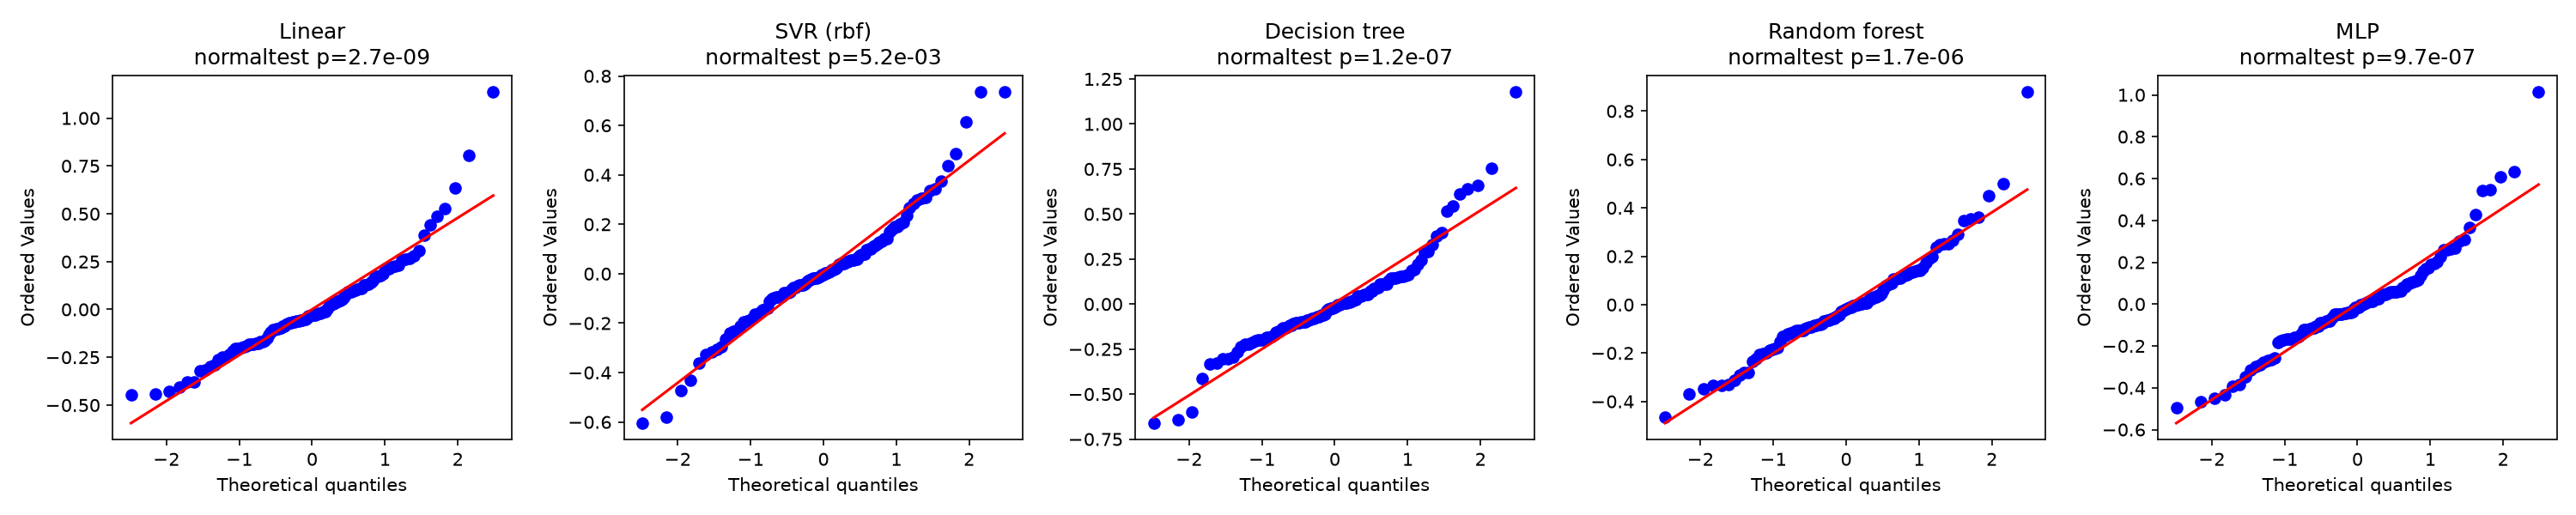
\includegraphics[width=\textwidth]{figs/qqplots.png}
  \end{center}
  \begin{center}
    \begin{tabular}{l r r r r}
      \hline
      Model & Std of residual & Skewness & Excess kurtosis & \texttt{normaltest} $p$ \\
      \hline
      Linear        & 0.246 & $+1.34$ & $+4.03$ & $2.7 \times 10^{-9}$ \\
      SVR (rbf)     & 0.226 & $+0.43$ & $+1.71$ & $5.2 \times 10^{-3}$ \\
      Decision tree & 0.265 & $+1.07$ & $+3.71$ & $1.2 \times 10^{-7}$ \\
      Random forest & 0.196 & $+0.94$ & $+3.08$ & $1.7 \times 10^{-6}$ \\
      MLP           & 0.234 & $+1.00$ & $+3.03$ & $9.7 \times 10^{-7}$ \\
      \hline
    \end{tabular}
  \end{center}
  Every model has $p < 0.01$, so at $\alpha = 0.05$ we reject normality for all five. The Q--Q plots agree: the points bend away from the line in the upper tail, and the residuals are right-skewed and heavy-tailed (positive skewness and excess kurtosis). Even the best-behaved model (SVR) is rejected. So the normality justification for squared error loss does not hold well on this dataset, which motivates the heavier-tailed $t$ loss in the regression part of Problem 5.
  \begin{lstlisting}[language=Python, numbers=none, xleftmargin=0pt, framexleftmargin=0pt, frame=none]
import numpy as np, pandas as pd, torch
import matplotlib; matplotlib.use("Agg")
import matplotlib.pyplot as plt
from scipy import stats
from sklearn.datasets import load_breast_cancer
from sklearn.model_selection import train_test_split, cross_val_predict
from sklearn.preprocessing import StandardScaler
from sklearn.pipeline import make_pipeline
from sklearn.linear_model import LinearRegression, LogisticRegression
from sklearn.svm import SVR
from sklearn.tree import DecisionTreeRegressor
from sklearn.ensemble import RandomForestRegressor
from sklearn.neural_network import MLPRegressor
from sklearn.metrics import accuracy_score, mean_absolute_error

SEED = 0
torch.manual_seed(SEED); np.random.seed(SEED)
torch.set_default_dtype(torch.float64)

ale = pd.read_csv("data/ale.csv")
X_ale = ale[["anchor_ratio", "trans_range", "node_density", "iterations"]].values
y_ale = ale["ale"].values

# ---------------------------------------------------------------- Problem 4
print("=" * 70, "\nProblem 4: normality of residuals\n" + "=" * 70)
models = {
    "Linear": make_pipeline(StandardScaler(), LinearRegression()),
    "SVR (rbf)": make_pipeline(StandardScaler(), SVR(C=10, epsilon=0.01)),
    "Decision tree": DecisionTreeRegressor(max_depth=5, random_state=SEED),
    "Random forest": RandomForestRegressor(n_estimators=200, random_state=SEED),
    "MLP": make_pipeline(StandardScaler(), MLPRegressor(hidden_layer_sizes=(64, 64), max_iter=5000, random_state=SEED)),
}
fig, axes = plt.subplots(1, len(models), figsize=(4 * len(models), 4))
for ax, (name, m) in zip(axes, models.items()):
    # out-of-fold predictions so residuals are not distorted by overfitting
    resid = y_ale - cross_val_predict(m, X_ale, y_ale, cv=10)
    k2, p = stats.normaltest(resid)
    print(f"{name:14s} resid mean={resid.mean():+.4f} std={resid.std():.4f} "
          f"skew={stats.skew(resid):+.2f} kurt={stats.kurtosis(resid):+.2f} "
          f"normaltest stat={k2:.2f} p={p:.2e}")
    stats.probplot(resid, dist="norm", plot=ax)
    ax.set_title(f"{name}\nnormaltest p={p:.1e}")
plt.tight_layout(); plt.savefig("figs/qqplots.png", dpi=150); plt.close()
  \end{lstlisting}
\end{solution}

\begin{exercise}[Classification]
  For this part, you will use the Breast Cancer Wisconsin dataset, which you can load using \texttt{sklearn.datasets.load\_breast\_cancer}. The dataset contains 30 features and a binary label. Begin by splitting the data (80/20) into a training and test set.

  As a baseline, use sklearn's implementation to train a logistic regression model on the training data and evaluate its accuracy on the test set, where accuracy is defined as the proportion of correctly classified observations.
  \begin{enumerate}[label=(\alph*)]
    \item Now you will implement a logistic regression model using a framework that supports automatic differentiation. Begin by defining a logistic regression model:
      \[
        f(x_i) = \sigma(w^T x_i + b)
      \]
      where $x_i$ are the features for observation $i$, $w$ are the weights, $b$ is the bias, and $\sigma$ is the sigmoid function. Next, define a function for the binary cross-entropy loss:
      \[
        L(y_i, f(x_i)) = -\left[y_i \log(f(x_i)) + (1 - y_i)\log(1 - f(x_i))\right]
      \]
      Use your chosen framework to implement this model and train it on the training data by minimizing the loss using SGD. Note that you may need to clip the output of the sigmoid function to avoid numerical instability. Evaluate the performance of your model on the test set. How does it compare to the baseline?
    \item Logistic regression uses the function $\sigma(z_i)$ to map the real-valued $z_i \coloneqq w^T x_i + b$ to a probability between 0 and 1. However, this is not the only way to map a real-valued output to a probability. Probit regression uses $\Phi(z_i)$, where $\Phi$ is the cumulative distribution function of the standard normal distribution. The model is then:
      \[
        f(x_i) = \Phi(w^T x_i + b)
      \]
      Implement a probit regression model. Using the same binary cross-entropy loss as before, train the model on the training data by minimizing the loss with SGD. As before, you may need to clip the output of the cumulative distribution function to avoid numerical instability. Evaluate the performance of your model on the test set. How does it compare to the baseline?
  \end{enumerate}
\end{exercise}
\begin{solution}
  I used PyTorch (\texttt{torch.optim.SGD}, minibatches of 32, learning rate $0.1$, 200 epochs, zero initialization, double precision) on an 80/20 stratified split (\texttt{random\_state}$=0$, 114 test points) with standardized features. The model outputs were clipped to $[10^{-7}, 1 - 10^{-7}]$ inside the loss, and probit used \texttt{torch.distributions.Normal(0, 1).cdf}. The full code is in \texttt{hw1\_code.py}.
  \begin{center}
    \begin{tabular}{l r}
      \hline
      Model & Test accuracy \\
      \hline
      sklearn \texttt{LogisticRegression} (baseline) & 0.9825 \\
      (a) Logistic regression, BCE + SGD             & 0.9825 \\
      (b) Probit regression, BCE + SGD               & 0.9825 \\
      \hline
    \end{tabular}
  \end{center}
  \begin{enumerate}[label=(\alph*)]
    \item The logistic regression trained by SGD matches the baseline at $98.25\%$ (112 of 114 correct).
    \item The probit regression also matches the baseline at $98.25\%$. Since $\Phi(z) \approx \sigma(1.7z)$, the two link functions differ mainly by a rescaling of $w$ and $b$, so it is unsurprising that they classify equally well here (the classification threshold $f = 0.5$ is the hyperplane $w^T x + b = 0$ in both cases).
  \end{enumerate}
  On this test set the three models are indistinguishable by accuracy.
  \begin{lstlisting}[language=Python, numbers=none, xleftmargin=0pt, framexleftmargin=0pt, frame=none]
# ---------------------------------------------------------------- helpers
def sgd_fit(loss_fn, params, Xtr, ytr, lr, epochs, batch=32, seed=SEED):
    """Minibatch SGD with torch.optim.SGD; loss_fn(params, X, y) -> scalar."""
    g = torch.Generator().manual_seed(seed)
    opt = torch.optim.SGD(params, lr=lr)
    n = len(Xtr)
    for _ in range(epochs):
        perm = torch.randperm(n, generator=g)
        for i in range(0, n, batch):
            idx = perm[i:i + batch]
            opt.zero_grad()
            loss_fn(params, Xtr[idx], ytr[idx]).backward()
            opt.step()
    return params

def to_t(*arrs):
    return [torch.tensor(a, dtype=torch.float64) for a in arrs]

# ---------------------------------------------------------------- Problem 5: classification
print("\n" + "=" * 70, "\nProblem 5: classification (Breast Cancer Wisconsin)\n" + "=" * 70)
Xc, yc = load_breast_cancer(return_X_y=True)
Xtr, Xte, ytr, yte = train_test_split(Xc, yc, test_size=0.2, random_state=SEED, stratify=yc)
sc = StandardScaler().fit(Xtr)
Xtr_s, Xte_s = sc.transform(Xtr), sc.transform(Xte)

base = LogisticRegression(max_iter=5000).fit(Xtr_s, ytr)
print(f"Baseline sklearn LogisticRegression test acc: {accuracy_score(yte, base.predict(Xte_s)):.4f}")

Xtr_t, Xte_t, ytr_t = to_t(Xtr_s, Xte_s, ytr.astype(float))
EPS = 1e-7
std_normal = torch.distributions.Normal(0.0, 1.0)

def make_bce(link):
    def loss(params, X, y):
        w, b = params
        f = link(X @ w + b).clamp(EPS, 1 - EPS)          # clip for stability
        return -(y * torch.log(f) + (1 - y) * torch.log(1 - f)).mean()
    return loss

for name, link in [("(a) Logistic (sigmoid)", torch.sigmoid), ("(b) Probit (Normal CDF)", std_normal.cdf)]:
    w = torch.zeros(Xtr_t.shape[1], requires_grad=True)
    b = torch.zeros(1, requires_grad=True)
    sgd_fit(make_bce(link), [w, b], Xtr_t, ytr_t, lr=0.1, epochs=200)
    with torch.no_grad():
        pred = (link(Xte_t @ w + b) > 0.5).numpy().astype(int)
    print(f"{name:25s} test acc: {accuracy_score(yte, pred):.4f}")
  \end{lstlisting}
\end{solution}

\addtocounter{exercise}{-1}
\begin{exercise}[Regression]
  For this part, you will use the average localization error (ALE) dataset from the previous question. Begin by splitting the data (80/20) into a training and test set.

  As a baseline, use sklearn's implementation to train a linear regression model on the training data and evaluate its performance on the test set using the mean absolute error.
  \begin{enumerate}[label=(\alph*)]
    \item Now you will implement a linear regression model using a framework that supports automatic differentiation. Begin by defining a linear regression model:
      \[
        f(x_i) = w^T x_i + b
      \]
      where $x_i$ are the features for observation $i$, $w$ are the weights, and $b$ is the bias. Next, define a function for the mean squared error loss:
      \[
        L(y_i, f(x_i)) = (y_i - f(x_i))^2
      \]
      Use your chosen framework to implement this model and train it on the training data by minimizing the loss with SGD. Evaluate the performance of your model on the test set. How does it compare to the baseline?
    \item Earlier you saw that the squared error loss can be derived from the assumption that the residuals of the fitted model should be (approximately) normal. However, the normal distribution has weak tails, so it is sensitive to outliers. An alternative is the t-distribution, which has heavier tails. The t-distribution is parameterized by the degrees of freedom $\nu$. When $\nu \to \infty$, the t-distribution converges to the standard normal distribution. The probability density function of the t-distribution is:
      \[
        p(y_i - f(x_i), \nu) = \frac{\Gamma\left(\frac{\nu+1}{2}\right)}{\sqrt{\nu\pi}\,\Gamma\left(\frac{\nu}{2}\right)} \left(1 + \frac{(y_i - f(x_i))^2}{\nu}\right)^{-\frac{\nu+1}{2}}
      \]
      where $\Gamma$ is the gamma function. The corresponding loss function is the negative log-likelihood:
      \[
        L(y_i, f(x_i)) = -\log p(y_i - f(x_i), \nu)
      \]
      For this exercise, use the t-distribution with $\nu = 5$. If you are using JAX, you can use \texttt{jax.scipy.stats.t.logpdf} to implement this loss function. If you are using PyTorch, you can use \texttt{torch.distributions.StudentT.log\_prob}.

      Use your chosen framework to implement a linear regression model and train it on the training data by minimizing this custom loss function with SGD. Evaluate the performance of your model on the test set. How does it compare to the baseline?
  \end{enumerate}
\end{exercise}
\begin{solution}
  I used the same setup as before: PyTorch with \texttt{torch.optim.SGD} (minibatches of 32, learning rate $0.05$, 300 epochs, $w = 0$, $b$ initialized to the mean of the training targets), an 80/20 split (\texttt{random\_state}$=0$, 22 test points) and standardized features. For (b) I wrote the loss as the explicit negative log-likelihood,
  \[
    -\log p(r, \nu) = -\log\Gamma\left(\tfrac{\nu+1}{2}\right) + \log\Gamma\left(\tfrac{\nu}{2}\right) + \tfrac{1}{2}\log(\nu\pi) + \tfrac{\nu+1}{2}\log\left(1 + \tfrac{r^2}{\nu}\right), \qquad r = y - f(x),
  \]
  with $\nu = 5$ (only the last term depends on the parameters).
  \begin{center}
    \small
    \begin{tabular}{l r r r r r r}
      \hline
      Model & $w_{\text{anchor}}$ & $w_{\text{range}}$ & $w_{\text{density}}$ & $w_{\text{iter}}$ & $b$ & Test MAE \\
      \hline
      sklearn baseline & $-0.054$ & $-0.072$ & $-0.293$ & $-0.214$ & 1.018 & 0.1921 \\
      (a) Squared error SGD & $-0.052$ & $-0.073$ & $-0.291$ & $-0.213$ & 1.019 & 0.1931 \\
      (b) Student-$t$ NLL + SGD & $-0.053$ & $-0.070$ & $-0.290$ & $-0.209$ & 1.016 & 0.1898 \\
      \hline
    \end{tabular}
  \end{center}
  (Weights are on standardized features, in the order \texttt{anchor\_ratio}, \texttt{trans\_range}, \texttt{node\_density}, \texttt{iterations}.)
  \begin{enumerate}[label=(\alph*)]
    \item SGD on the squared error reaches a test MAE of $0.1931$ versus $0.1921$ for the baseline. This is expected, since both minimize the same convex objective and SGD converges to (a neighborhood of) the least squares solution; the fitted coefficients agree with the closed-form ones to about two decimals.
    \item SGD on the Student-$t$ loss reaches a test MAE of $0.1898$, which is about $1\%$ lower than the baseline. This is in the direction one would expect from the heavy-tailed residuals found in Problem 4, since the $t$ loss grows only logarithmically in the residual and so downweights outliers. However, the difference is tiny, and with only 22 test points it is well within noise, so I would conclude that the model performs about the same as the baseline.
  \end{enumerate}
  \begin{lstlisting}[language=Python, numbers=none, xleftmargin=0pt, framexleftmargin=0pt, frame=none]
# ---------------------------------------------------------------- Problem 5: regression
print("\n" + "=" * 70, "\nProblem 5: regression (ALE)\n" + "=" * 70)
Xtr, Xte, ytr, yte = train_test_split(X_ale, y_ale, test_size=0.2, random_state=SEED)
sc = StandardScaler().fit(Xtr)
Xtr_s, Xte_s = sc.transform(Xtr), sc.transform(Xte)

base = LinearRegression().fit(Xtr_s, ytr)
print(f"Baseline sklearn LinearRegression test MAE: {mean_absolute_error(yte, base.predict(Xte_s)):.4f}")

Xtr_t, Xte_t, ytr_t = to_t(Xtr_s, Xte_s, ytr)
NU = 5.0

def mse_loss(params, X, y):
    w, b = params
    return ((y - (X @ w + b)) ** 2).mean()

def t_nll(params, X, y):
    w, b = params
    r = y - (X @ w + b)
    # -log p(r; nu) = -lgamma((nu+1)/2) + lgamma(nu/2) + 0.5 log(nu pi) + (nu+1)/2 log(1 + r^2/nu)
    return (-torch.lgamma(torch.tensor((NU + 1) / 2)) + torch.lgamma(torch.tensor(NU / 2))
            + 0.5 * np.log(NU * np.pi) + (NU + 1) / 2 * torch.log1p(r ** 2 / NU)).mean()

for name, loss in [("(a) Squared error + SGD", mse_loss), (f"(b) Student-t (nu={NU:g}) NLL + SGD", t_nll)]:
    w = torch.zeros(Xtr_t.shape[1], requires_grad=True)
    b = torch.tensor([float(ytr.mean())], requires_grad=True)   # start at mean of y
    sgd_fit(loss, [w, b], Xtr_t, ytr_t, lr=0.05, epochs=300)
    with torch.no_grad():
        mae = (Xte_t @ w + b - torch.tensor(yte)).abs().mean().item()
    print(f"{name:36s} test MAE: {mae:.4f}   w={w.detach().numpy().round(3)} b={b.item():.3f}")
  \end{lstlisting}
\end{solution}

\end{document}
